\documentclass[12pt,a4paper,twoside,openany]{book}
\usepackage{graphicx}
\usepackage{setspace} % espaciado doble para texto, simple para pies de página, subtítulos, etc.
\usepackage{natbib} % sustituto de 'hypernat' que funciona en Windows.
\usepackage[spanish]{babel}
\usepackage[utf8]{inputenc}
\usepackage{color}
\usepackage{hhline} % estilos extendidos para tablas
\usepackage{multirow}
\usepackage{subfigure}
\usepackage{acronym}
\usepackage{hyperref}
\usepackage{amsmath,amssymb}
\usepackage{fancyhdr}
\usepackage{epsfig, amsmath}
\usepackage{algorithm}
\usepackage{algorithmic}
\usepackage[T1]{fontenc}
\usepackage{lmodern}
\usepackage{microtype}
\usepackage{tabularx}
\usepackage{longtable}
\usepackage{array}

\let\cleardoublepage\clearpage

% configuraciones generales
\hypersetup{
linktocpage=true,
colorlinks=true,
linkcolor=blue,
citecolor=blue,
}
\definecolor{Hgray}{gray}{0.6}

\newenvironment{definition}[1][Definición]{\begin{trivlist}
\item[\hskip \labelsep {\bfseries #1}]}{\end{trivlist}}

\setlength{\topmargin}{0cm}
\setlength{\textheight}{23cm}
\setlength{\textwidth}{17cm}
\setlength{\oddsidemargin}{0cm}
\setlength{\evensidemargin}{0cm}
\setlength{\headheight}{1cm}

% indica que las 'sub-sub-secciones' están numeradas y aparecen en el índice
\setcounter{secnumdepth}{3}
\setcounter{tocdepth}{2}

% configuraciones para código
\renewcommand{\algorithmicrequire}{\textbf{Entrada:}}
\renewcommand{\algorithmicensure}{\textbf{Salida:}}

%%%%%%%%%%%%
% DOCUMENTO %
%%%%%%%%%%%%
\begin{document}

\setcounter{section}{0} % Restablece el contador de sección a 0 al inicio del documento
\renewcommand{\thesection}{\arabic{section}} % Cambia el esquema de numeración de sección

\pagenumbering{arabic}

\hypersetup{pageanchor=true}

% portada
\newpage
\thispagestyle{empty}

\baselineskip 2em

%\vspace*{1cm}

\centerline{
\includegraphics[width=0.6\textwidth]{images/UOC-logo}}
\begin{center}
\textsc{Universitat Oberta de Catalunya (UOC) \\
 Máster Universitario en Ciencia de Datos (\textit{Data Science})\\}

%\centerline {\pic{UOC}{4cm}}

\vspace*{1.5cm}

\textsc{\Large TRABAJO FINAL DE MÁSTER}

\vspace*{0.5cm}

\textsc{\large Área: Reinforced Learning}


%\textbf{\Huge VirtualTechLab Model: }

\vspace*{2.0cm}

\textbf{\Large Impacto de la complejidad de las observaciones en el rendimiento de algoritmos de Aprendizaje por Refuerzo en un entorno Pacman}

\vspace{2.5cm}
\baselineskip 1em

\baselineskip 2em
-----------------------------------------------------------------------------\\
Autor:      Alejandro Suau Ruiz\\
Tutor:      Marc Borras Camarasa\\
Profesor:   David Masip Rodó\\
-----------------------------------------------------------------------------\\
\vspace*{1.5cm}
Palma de Mallorca, \today

\end{center}

\newpage
\pagestyle{empty}
\hfill

\newpage
% resumen
\hypersetup{pageanchor=false}
\pagenumbering{roman} 
\setcounter{page}{1} 
\pagestyle{plain}

%%%%%%%%%%%%%%%%
%%% CREDITOS %%%
%%%%%%%%%%%%%%%%
\chapter*{Créditos/Copyright}

Una página con la especificación de créditos/copyright para el proyecto (ya sea aplicación por un lado y documentación por el otro, o unificadamente), así como la del uso de marcas, productos o servicios de terceros (incluidos códigos fuente). Si una persona diferente al autor colaboró en el proyecto, tiene que quedar explicitada su identidad y qué hizo.

A continuación se ejemplifica el caso más habitual, aunque se puede modificar por cualquier otra alternativa:

\vspace{1cm}

\begin{figure}[ht]
    \centering
	
\includegraphics[scale=1]{images/license.png}
\end{figure}

Esta obra está sujeta a una licencia de Reconocimiento -  NoComercial - SinObraDerivada

\href{https://creativecommons.org/licenses/by-nc-nd/3.0/es/}{3.0 España de CreativeCommons}.

%%%%%%%%%%%%%
%%% FICHA %%%
%%%%%%%%%%%%%
\chapter*{FICHA DEL TRABAJO FINAL}

\begin{table}[ht]
	\centering{}
	\renewcommand{\arraystretch}{2}
	\begin{tabular}{r | l}
		\hline
		Título del trabajo: & Impacto de la complejidad de las observaciones en el rendimiento de algoritmos de Aprendizaje por Refuerzo en un entorno Pacman\\
		\hline
        Nombre del autor: & Alejandro Suau Ruiz\\
		\hline
        Nombre del colaborador/a docente: & Marc Borras Camarasa\\
		\hline
        Nombre del PRA: & David Masip Rodó\\
		\hline
        Fecha de entrega (mm/aaaa): & 01/2026\\
		\hline
        Titulación o programa: & Máster Universitario de Data Science\\
		\hline
        Área del Trabajo Final: & Reinforced Learning\\
		\hline
        Idioma del trabajo: & Español\\
		\hline
        Palabras clave & Aprendizaje por refuerzo, Complejidad del estado, Pacman\\
		\hline
	\end{tabular}
\end{table}

%%%%%%%%%%%%%%%%%%%
%%% DEDICATORIA %%%
%%%%%%%%%%%%%%%%%%%
\chapter*{Dedicatoria/Cita}

Breves palabras de dedicatoria y/o una cita.

%%%%%%%%%%%%%%%%%%%
%%% Agradecimientos %%%
%%%%%%%%%%%%%%%%%%%
\chapter*{Agradecimientos}

Si se considera oportuno, mencionar a las personas, empresas o instituciones que hayan contribuido en la realización de este proyecto.

%%%%%%%%%%%%%%%%
%%% ABSTRACT%%%
%%%%%%%%%%%%%%%%
\chapter*{Abstract}
\addcontentsline{toc}{chapter}{Abstract}

\onehalfspacing

This work investigates how the complexity of state representation affects the performance of reinforcement learning algorithms in a simplified Pacman environment. The central idea is that an agent’s success depends not only on the algorithm itself but also on the quality and richness of the information it receives from the environment. To analyze this, we designed a set of progressively more complex observation spaces, ranging from the basic positions of the player and the ghost to configurations that include the presence and duration of power-ups and the distribution of coins across quadrants.
Experiments were carried out using widely adopted algorithms such as PPO, A2C, and DQN, implemented with the Stable-Baselines3 library. Controlled training with different random seeds and consistent performance metrics allowed us to compare both learning speed and the stability of the learned policies.
The results show that increasing state complexity does not always lead to better performance: in some cases, the additional information introduces noise and hinders convergence. However, for specific configurations, the agent was able to exploit the extra information to achieve more robust behavior.
In conclusion, the project highlights the importance of observation design in the success of reinforcement learning agents, stressing the need to balance simplicity and expressiveness depending on the task and the chosen algorithm.

\vspace{1.5cm}

\textbf{Keywords}: Reinforcement learning, State complexity, Pacman, Stable-Baselines3, Gymnasium

%%%%%%%%%%%%%%%%
%%% RESUMEN    %%%
%%%%%%%%%%%%%%%%

\chapter*{Resumen}
\addcontentsline{toc}{chapter}{Resumen}

\onehalfspacing

Este trabajo explora cómo la complejidad de la representación del estado influye en el rendimiento de los algoritmos de aprendizaje por refuerzo en un entorno simplificado de Pacman. Partimos de la premisa de que un agente no aprende únicamente por el algoritmo empleado, sino también por la calidad y la riqueza de la información que percibe del entorno. Para analizarlo, hemos diseñado un conjunto de observaciones progresivamente más complejas, desde la posición básica de jugador y fantasma, hasta configuraciones que incluyen la presencia y duración de comodines o la distribución de monedas por cuadrantes.
La experimentación se ha llevado a cabo con algoritmos ampliamente utilizados, como PPO, A2C y DQN, implementados con la librería Stable-Baselines3. Se han realizado entrenamientos controlados con semillas distintas y métricas de rendimiento homogéneas, lo que ha permitido comparar tanto la velocidad de aprendizaje como la estabilidad de las políticas aprendidas.
Los resultados muestran que un aumento en la complejidad del estado no garantiza siempre un mejor desempeño: en ciertos casos, la mayor riqueza de información introduce ruido y dificulta la convergencia. Sin embargo, para determinadas configuraciones el agente logra aprovechar la información adicional y alcanzar un comportamiento más robusto.
En conclusión, el proyecto confirma la relevancia del diseño de observaciones en el éxito de un agente de aprendizaje por refuerzo, subrayando la necesidad de equilibrar simplicidad y expresividad en función del objetivo y del algoritmo empleado.


\vspace{1.5cm}

\textbf{Palabras clave}: Aprendizaje por refuerzo, Complejidad del estado, Pacman, Stable-Baselines3, Gymnasium
\newpage

\pagestyle{fancy}
\renewcommand{\chaptermark}[1]{ \markboth{#1}{}}
\renewcommand{\sectionmark}[1]{\markright{ \thesection.\ #1}}
\lhead[\fancyplain{}{\bfseries\thepage}]{\fancyplain{}{\bfseries\rightmark}}
\rhead[\fancyplain{}{\bfseries\leftmark}]{\fancyplain{}{\bfseries\thepage}}
\cfoot{}

% tabla de contenidos
\cleardoublepage
\phantomsection
\addcontentsline{toc}{chapter}{Índice}
\tableofcontents
% lista de figuras
\cleardoublepage
\phantomsection
\addcontentsline{toc}{chapter}{Lista de Figuras}
\listoffigures
% lista de tablas
\cleardoublepage
\phantomsection
\addcontentsline{toc}{chapter}{Lista de Tablas}
\listoftables

\thispagestyle{empty}

\pagenumbering{arabic}

\pagestyle{fancy}
\renewcommand{\chaptermark}[1]{ \markboth{#1}{}}
\renewcommand{\sectionmark}[1]{\markright{ \thesection.\ #1}}
\lhead[\fancyplain{}{\bfseries\thepage}]{\fancyplain{}{\bfseries\rightmark}}
\rhead[\fancyplain{}{\bfseries\leftmark}]{\fancyplain{}{\bfseries\thepage}}
\cfoot{}

\onehalfspacing

% capítulos del documento
\chapter{Introducción}
\label{chapter:introduccion}


%%% SECTION
\section{Descripción general del problema}

En la actualidad, los procesos de minería de datos requieren grandes cantidades de datos, que en muchas ocasiones contienen información personal y privada de usuarios o personas. Aunque se realicen procesos básicos de anonimización sobre los datos, es decir, eliminación de los nombres u otros identificadores clave, existen multitud de técnicas de re-identificación que permiten volver a identificar a un usuario dentro de este conjunto de datos. En la Figura \ref{fig:context-anoni1} se presenta un mapa donde es posible contextualizar los procesos de anonimización y re-identificación dentro de un proceso de minería de datos.

\begin{figure}
	\centering
	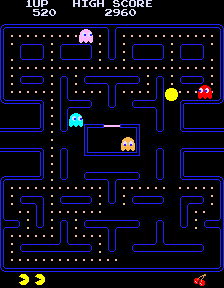
\includegraphics[width=0.6\textwidth]{figs/image1.png}
	\caption{Pie de la imagen.}
	\label{fig:context-anoni1}
\end{figure}

\subsection{Ejemplo de subsection}

Aunque se han realizado importantes avances en preservación de la privacidad en publicación de datos, tales como el modelo \textit{k}-anonymity \cite{Sweeney:2002}.

Un ejemplo de pseudo-código se puede encontrar en el Código \ref{code:RandomSwitch-1}

\begin{algorithm}
	\caption{Pseudocódigo del algoritmo \textit{Random Switch}}
	\label{code:RandomSwitch-1}
	\begin{algorithmic}
		\REQUIRE{El grafo original $G$ y el porcentaje de anonimización $p$ que se desea aplicar.}
		\ENSURE{El grafo $G$ anonimizado.}
		\STATE $num = round(G.num\_edges() * p)$
		\STATE $i = 0$
		\WHILE {$i < num$}
		\STATE {$e_{1} = G.random\_edge()$}
		\STATE $e_{2} = G.random\_edge()$
		\STATE $new\_e_{1} = (e_{1}.origen, e_{2}.origen)$
		\STATE $new\_e_{2} = (e_{1}.destino, e_{2}.destino)$
		\IF {$!G.exist(new\_e_{1})$ \AND $!G.exist(new\_e_{2})$}
		\STATE $G.add\_edge(new\_e_{1})$
		\STATE $G.add\_edge(new\_e_{2})$
		\STATE $G.delete\_edge(e_{1})$
		\STATE $G.delete\_edge(e_{2})$
		\STATE $i=i+1$
		\ENDIF
		\ENDWHILE
		\RETURN $G$
	\end{algorithmic}
\end{algorithm}

Un ejemplo de tabla se puede ver en la Tabla \ref{table:ejemplo_vertex_refi_query}

\begin{table}
	\centering{}
	\begin{tabular}{ l || c | c | l }
		\hline
		Node ID & $\mathcal{H}_{0}$ & $\mathcal{H}_{1}$ & $\mathcal{H}_{2}$ \\
		\hline
		\hline
		Alice & $\epsilon$ & 1 & \{4\}  \\
		\hline
		Bob & $\epsilon$ & 4 & \{1, 1, 4, 4\}  \\
		\hline
		Carol & $\epsilon$ & 1 & \{4\}  \\
		\hline
		Dave & $\epsilon$ & 4 & \{2, 4, 4, 4\}  \\
		\hline
		Ed & $\epsilon$ & 4 & \{2, 4, 4, 4\}  \\
		\hline
		Fred & $\epsilon$ & 2 & \{4, 4\}  \\
		\hline
		Greg & $\epsilon$ & 4 & \{2, 2, 4, 4\}  \\
		\hline
		Harry & $\epsilon$ & 2 & \{4, 4\}  \\
		\hline
	\end{tabular}
	\caption{\textit{Vertex refinement queries}.}
	\label{table:ejemplo_vertex_refi_query}
\end{table}

\chapter{Estado del arte}

\section{Fundamentos del Aprendizaje por Refuerzo}

El \textit{Aprendizaje por Refuerzo} (Reinforcement Learning, RL) constituye una de las ramas más relevantes del aprendizaje automático orientadas a la toma de decisiones secuenciales bajo incertidumbre. En este paradigma, un agente interactúa con un entorno mediante un proceso de prueba y error, buscando maximizar una recompensa acumulada a largo plazo. Formalmente, este proceso se modela como un \textit{Proceso de Decisión de Markov} (MDP), definido por el conjunto $(S, A, P, R, \gamma)$, donde $S$ representa el espacio de estados, $A$ el conjunto de acciones posibles, $P(s'|s,a)$ la función de transición de estados, $R(s,a)$ la función de recompensa y $\gamma \in [0,1]$ el factor de descuento que pondera la importancia de las recompensas futuras \citep{SuttonBarto2018}.

El objetivo de un agente es encontrar una política óptima $\pi^*(a|s)$ que maximice el retorno esperado:

\begin{equation}
G_t = \mathbb{E}\left[\sum_{k=0}^{\infty} \gamma^k r_{t+k+1}\right],
\end{equation}

donde $r_{t+k+1}$ representa la recompensa obtenida $k$ pasos después del tiempo $t$.  
A diferencia del aprendizaje supervisado, el RL no dispone de un conjunto fijo de ejemplos etiquetados: el conocimiento se adquiere mediante la experiencia directa con el entorno.  

Los algoritmos de RL pueden clasificarse en dos grandes familias.  
Los \textbf{métodos basados en valor} estiman la utilidad esperada de los estados o pares estado–acción a través de funciones $V(s)$ o $Q(s,a)$, como en los algoritmos Q-Learning o SARSA.  
Por otro lado, los \textbf{métodos basados en política} parametrizan directamente la política $\pi_\theta(a|s)$ mediante un modelo (típicamente una red neuronal) y optimizan sus parámetros $\theta$ a partir del gradiente de la recompensa esperada.  
La combinación de ambos enfoques da lugar a los métodos \textbf{actor-crítico}, donde un componente (\textit{crítico}) estima el valor de los estados y otro (\textit{actor}) actualiza la política en función de dicha estimación.

En este marco, la \textbf{definición del estado} $s_t$ es un factor determinante.  
La información que el agente percibe condiciona su capacidad para generalizar, explorar y aprender políticas efectivas. Una representación excesivamente simple puede ocultar detalles relevantes del entorno, mientras que una observación demasiado compleja puede introducir ruido, ralentizar la convergencia y requerir redes de mayor capacidad.  
Por ello, la \textbf{complejidad del estado observado} constituye una variable crítica para la eficiencia del aprendizaje, y su análisis es el eje central del presente trabajo.

\vspace{0.5em}

\section{Avances en Deep Reinforcement Learning}

La integración del aprendizaje por refuerzo con redes neuronales profundas dio lugar al \textit{Aprendizaje por Refuerzo Profundo} (Deep Reinforcement Learning, DRL), que permite aproximar funciones de valor o políticas directamente a partir de observaciones de alta dimensión, como imágenes o secuencias temporales.  
Este enfoque ha sido clave para ampliar el alcance del RL a entornos complejos donde las representaciones manuales del estado resultan inviables \citep{Mnih2015}.

El punto de inflexión en la historia del DRL se produjo con el algoritmo \textbf{Deep Q-Network (DQN)} desarrollado por Mnih et al. \citeyearpar{Mnih2015}, que combinó Q-Learning con redes convolucionales para aprender directamente a partir de píxeles en entornos Atari.  
Entre sus principales innovaciones destacan dos mecanismos fundamentales:  
(1) el \textit{Experience Replay}, que almacena transiciones $(s,a,r,s')$ y las reutiliza en mini-lotes aleatorios para romper la correlación temporal entre muestras, y  
(2) la \textit{Target Network}, una red secundaria que se actualiza con menor frecuencia y estabiliza el aprendizaje.  
DQN demostró por primera vez que un agente podía alcanzar rendimientos comparables a los humanos en una variedad de videojuegos, marcando el inicio del auge del DRL.

A partir de DQN surgieron numerosas variantes orientadas a mejorar la estabilidad y eficiencia, como \textit{Double DQN}, \textit{Dueling DQN} o \textit{Rainbow DQN}, que integran mecanismos de priorización de experiencias, ponderación de ventajas o combinación de aprendizajes multiobjetivo.  
Sin embargo, estos métodos basados en valor presentan limitaciones en espacios de acción continuos, donde la búsqueda discreta de la acción óptima resulta impracticable.

Para abordar esas limitaciones, se desarrollaron los \textbf{métodos actor-crítico}, que combinan la estimación de valor y la política en un mismo marco.  
Uno de los más representativos es el \textit{Advantage Actor-Critic (A2C)}, versión síncrona del A3C (\textit{Asynchronous Advantage Actor-Critic}) \citep{Mnih2016}.  
En A2C, varios agentes ejecutan episodios en paralelo compartiendo una política común, lo que reduce la varianza del gradiente y acelera la convergencia.  
La estimación de la ventaja $A(s,a) = Q(s,a) - V(s)$ permite medir cuánto mejor resulta ejecutar una acción respecto a la media de acciones posibles en un estado dado.

Posteriormente, Schulman et al. \citeyearpar{Schulman2017} introdujeron el algoritmo \textbf{Proximal Policy Optimization (PPO)}, que se consolidó como uno de los métodos más utilizados por su equilibrio entre simplicidad y robustez.  
PPO limita el cambio de la política mediante una función de recorte (\textit{clipping}) que evita actualizaciones excesivas, garantizando una mejora estable y controlada.  
Su implementación eficiente en librerías como Stable-Baselines3 \citep{Raffin2021} ha favorecido su adopción tanto en investigación como en aplicaciones prácticas.

En síntesis, DQN, A2C y PPO representan tres paradigmas complementarios del DRL:  
\begin{itemize}
    \item \textbf{DQN:} aprendizaje basado en valor, idóneo para espacios de acción discretos, pero sensible a la estructura de la observación.  
    \item \textbf{A2C:} enfoque actor-crítico que equilibra exploración y estabilidad mediante aprendizaje paralelo.  
    \item \textbf{PPO:} optimización de políticas próximas, robusta ante variaciones en la dimensionalidad del estado.  
\end{itemize}

Estas características los convierten en candidatos idóneos para analizar de forma comparativa cómo la \textbf{complejidad de la observación} afecta el rendimiento del aprendizaje, manteniendo constante la dinámica y la recompensa del entorno.  

\vspace{0.5em}

\section{Síntesis y vacíos detectados}

La revisión de la literatura evidencia que, aunque el Aprendizaje por Refuerzo Profundo ha experimentado avances notables en la última década, gran parte de los esfuerzos se ha centrado en la \textbf{optimización de los algoritmos} —ya sea mediante arquitecturas, estrategias de exploración o funciones de pérdida—, mientras que el impacto de la representación del estado ha recibido menor atención.  
En la mayoría de los estudios, el espacio de observación se trata como una variable fija del entorno, sin evaluar de manera sistemática cómo su complejidad o riqueza informacional influye en la eficacia del aprendizaje.

En respuesta a esta limitación, han surgido líneas de investigación como el \textit{State Representation Learning} (SRL), que busca aprender representaciones latentes más compactas y relevantes para la toma de decisiones \citep{Lesort2018,Ha2018,Hafner2020}.  
Estos trabajos utilizan modelos generativos o redes autoencoder para capturar información útil en espacios de menor dimensión, lo que facilita la generalización y reduce el coste computacional.  
No obstante, la mayoría de enfoques SRL se orientan a la \textbf{construcción automática de representaciones} y no al estudio explícito del efecto de distintos niveles de complejidad observacional sobre el proceso de aprendizaje.

De forma complementaria, los estudios sobre entornos parcialmente observables \citep{Hausknecht2015} han puesto de manifiesto cómo la falta de información puede limitar la convergencia y provocar políticas subóptimas.  
Sin embargo, apenas existen análisis controlados sobre el efecto contrario: cómo el exceso de información o la redundancia en el estado pueden degradar el rendimiento o ralentizar la convergencia.  

Los entornos más utilizados como \textit{benchmarks}, tales como Atari o MuJoCo, ofrecen espacios de observación fijos, lo que impide aislar experimentalmente esta variable.  
En años recientes, entornos modulares como \textit{MiniGrid} \citep{ChevalierBoisvert2018} o \textit{ProcGen} \citep{Cobbe2020} han permitido cierta variabilidad estructural, aunque su propósito principal ha sido evaluar la capacidad de generalización entre tareas, no la complejidad del estado como tal.

En este contexto, se identifica un vacío experimental relevante: la ausencia de estudios que analicen de forma controlada la relación entre la \textbf{complejidad del espacio de observación} y el rendimiento de distintos algoritmos de RL manteniendo constantes las dinámicas, recompensas y reglas del entorno.  

El presente trabajo busca contribuir a llenar ese vacío mediante el desarrollo de un entorno propio, \textit{SimplePacmanEnv}, inspirado en el clásico juego Pac-Man.  
Dicho entorno permite parametrizar el nivel de información observable, desde representaciones mínimas (posición del agente y del fantasma) hasta configuraciones enriquecidas con comodines, distribución de monedas o vistas tipo imagen.  
Esta configuración experimental posibilita evaluar empíricamente cómo la cantidad y naturaleza de la información percibida influyen en la estabilidad del entrenamiento, la velocidad de convergencia y la calidad final de la política aprendida.

En conjunto, este análisis pretende aportar una visión empírica y reproducible sobre el equilibrio entre \textbf{simplicidad y expresividad} en el diseño de observaciones, contribuyendo así a una comprensión más profunda del papel de la percepción en el rendimiento de los agentes de aprendizaje por refuerzo.


\chapter{Planificación del proyecto}

\section{Recursos necesarios}

A continuación se detallan los recursos técnicos, de software y humanos requeridos para el desarrollo del proyecto. La selección de estos recursos se ha realizado considerando la naturaleza computacional del trabajo y la necesidad de garantizar reproducibilidad y eficiencia durante el proceso experimental.

\begin{longtable}{>{\bfseries}p{3.5cm} p{10cm}}
Tipo de recurso & Descripción \\ \hline
Hardware & Ordenador personal con CPU multinúcleo (Intel i7 o equivalente), 16 GB de RAM y GPU NVIDIA opcional para acelerar el entrenamiento de redes neuronales. \\
Software & Sistema operativo Linux/Windows, Python 3.10+, librerías \textit{Gymnasium}, \textit{Stable-Baselines3}, \textit{NumPy}, \textit{Matplotlib} y \textit{TensorBoard} para la monitorización de entrenamientos. \\
Control de versiones & Repositorio privado en GitHub para gestionar código, scripts y documentación. \\
Datos y experimentos & No se requieren datasets externos: los datos se generan de forma simulada a través del entorno \texttt{SimplePacmanEnv}. \\
Apoyo académico & Tutorías con el tutor del TFM y revisión periódica según las fases definidas en las PEC. \\
\end{longtable}

\section{Planificación temporal y tareas}

El proyecto se organiza siguiendo las fases de los módulos del TFM (de M1 a M5), que marcan los hitos principales de evaluación continua. Cada fase combina tareas de análisis, desarrollo y documentación.

\begin{longtable}{|>{\bfseries}p{3cm}|p{2.8cm}|p{7.8cm}|p{2.8cm}|}
\hline
Fase / Módulo & Periodo aproximado & Descripción de tareas principales & Hito asociado \\
\hline
M1 -- Definición y planificación del TFM & 25 sep -- 12 oct 2025 & 
\begin{itemize}
\item Definir objetivos y alcance del proyecto.
\item Revisar la viabilidad técnica y ética.
\item Elaborar propuesta inicial y planificación.
\end{itemize} & Entrega M1 (12 oct) \\ \hline

M2 -- Estado del arte y fundamentos teóricos & 13 oct -- 2 nov 2025 &
\begin{itemize}
\item Revisión bibliográfica sobre aprendizaje por refuerzo, entornos Gym y algoritmos A2C, PPO y DQN.
\item Identificación de trabajos similares y justificación del enfoque experimental.
\end{itemize} & Entrega M2 (2 nov) \\ \hline

M3 -- Diseño e implementación del sistema & 3 nov -- 14 dic 2025 &
\begin{itemize}
\item Implementar el entorno \texttt{SimplePacmanEnv}.
\item Desarrollar scripts de entrenamiento (\texttt{train\_a2c.py}, \texttt{train\_ppo.py}, \texttt{train\_dqn.py}).
\item Validar funcionalidad y reproducibilidad.
\item Documentar el código.
\end{itemize} & Entrega M3 (14 dic) \\ \hline

M4 -- Redacción y análisis de resultados & 22 dic -- 28 dic 2025 &
\begin{itemize}
\item Entrenar los modelos con distintas configuraciones de observación.
\item Analizar resultados y elaborar gráficas comparativas.
\item Redactar la memoria y preparar la presentación audiovisual.
\end{itemize} & Entrega M4 (21--28 dic); vídeo: 6 ene 2026 \\ \hline

M5 -- Defensa y cierre del proyecto & 9 ene -- 30 ene 2026 &
\begin{itemize}
\item Entrega final de la documentación al tribunal.
\item Presentación y defensa pública del trabajo.
\item Revisión y cierre de la memoria.
\end{itemize} & Entrega y defensa (9--30 ene) \\ \hline
\end{longtable}

\section{Diagrama de Gantt simplificado}

El diagrama de Gantt que se presenta a continuación resume de forma visual la distribución temporal de las actividades y su solapamiento a lo largo del semestre académico. Cada marca indica aproximadamente una semana de dedicación dentro del mes correspondiente.

\begin{center}
\renewcommand{\arraystretch}{1.2}
\begin{tabular}{|>{\bfseries}p{6cm}|c|c|c|c|c|c|}
\hline
Actividad / Mes & Sep & Oct & Nov & Dic & Ene & Feb \\
\hline
Definición y planificación (M1) & XX & X &  &  &  &  \\
\hline
Estado del arte (M2) &  & XXX &  &  &  &  \\
\hline
Diseño e implementación (M3) &  & X & XXXX & X &  &  \\
\hline
Análisis y redacción (M4) &  &  &  & XXX & X &  \\
\hline
Defensa y cierre (M5) &  &  &  &  & XXX & X \\
\hline
\end{tabular}
\end{center}

\noindent
\textit{Nota:} cada ``X'' representa aproximadamente una semana de trabajo dentro del mes correspondiente.


\section{Hitos principales del proyecto}

Finalmente, se resumen los hitos más relevantes del proyecto, vinculados a las Pruebas de Evaluación Continua (PEC) y a las entregas oficiales del calendario académico. Estos hitos marcan los puntos de control que estructuran el avance del trabajo desde su definición inicial hasta la defensa final.

\begin{longtable}{|>{\bfseries}p{2.8cm}|p{3cm}|p{9cm}|}
\hline
Hito & Fecha aproximada & Descripción \\
\hline
H1 -- Definición del TFM (PEC1) & 12 oct 2025 & Entrega del documento de definición y planificación del TFM. \\ \hline
H2 -- Estado del arte (PEC2) & 2 nov 2025 & Entrega del marco teórico y análisis del contexto del trabajo. \\ \hline
H3 -- Implementación (PEC3) & 14 dic 2025 & Finalización del entorno funcional y de los scripts de entrenamiento. \\ \hline
H4 -- Redacción preliminar y final (PEC4) & 21--28 dic 2025 & Entrega del documento completo del TFM y del vídeo de presentación. \\ \hline
H5 -- Defensa final (PEC5) & 30 ene 2026 & Presentación pública y defensa del trabajo ante el tribunal. \\ \hline
\end{longtable}


\section{Resumen de los productos del proyecto}

No es necesario describir cada producto en detalle: esto se hará en los capítulos restantes del proyecto.

\section{Breve descripción de los demás capítulos del informe}

Breve descripción de los contenidos de cada capítulo y su relación con el resto del proyecto.

\section{Métodos y recursos}

En estas secciones, es necesario describir:

\begin{itemize}
    \item Los aspectos más relevantes del diseño y desarrollo del proyecto.
    \item La metodología utilizada en el proceso de desarrollo, describiendo las alternativas posibles, las decisiones que se han tomado y los criterios utilizados para tomar estas decisiones.
    \item Una descripción de los productos que se han creado.
\end{itemize}

La estructura de estas secciones puede cambiar según el tipo de proyecto que se esté desarrollando.

\section{Resultados}

Describa los resultados obtenidos utilizando la metodología descrita anteriormente.

\section{Conclusiones y trabajo futuro}

Esta sección debe incluir lo siguiente:

\begin{itemize}
    \item Una descripción de las conclusiones del trabajo.
    \item Una evaluación crítica del grado de logro de los objetivos iniciales.
    \item Una evaluación crítica de la planificación y metodología utilizadas en el proyecto.
    \item Considerando los desafíos de sostenibilidad, diversidad y ético-sociales vinculados al proyecto.
    \item Una discusión de temas para trabajo futuro potencial que no se hayan explorado en este proyecto.
\end{itemize}

\section{Glosario}

Definición de los términos y acrónimos más relevantes utilizados en este informe.

% bibliografía
\nocite{*}
\addcontentsline{toc}{chapter}{Bibliografía}
\bibliographystyle{plainnat}
\bibliography{referencias}

\section{Anexos}

\begin{enumerate}
    \item -
\end{enumerate}

\end{document}
